\chapter{Fuentes de la revisión exploratoria (Elicit Pro)}\label{cap:anexo1}

Se recoge el conjunto de \textbf{fuentes} identificadas en la búsqueda exploratoria (Elicit Pro), conservando su \textbf{numeración original}. Los índices que aparecen entre corchetes en la tabla de análisis del Capítulo~2 (Tabla~\ref{tab:analisis}) remiten al número correspondiente de este listado.

{\footnotesize
\begin{enumerate}\setlength{\itemsep}{2pt}
\item Xu B, Su J, Wang W (2018) An expanding balloon: a small universe. The Physical Educator. \url{https://doi.org/10.1088/1361-6552/aad71f}
\item Suárez Á (2025) Exploring cosmology: a simple experiment to illustrate the cosmological principle and the Hubble–Lemaître Law. The Physical Educator. \url{https://doi.org/10.1088/1361-6552/adac24}
\item Marshall O, Tojeiro R, Weijmans A (2022) Demonstrating cosmological and Doppler redshift in the classroom. 4th Symposium on Space Educational Activities. \url{https://doi.org/10.5821/conference-9788419184405.098}
\item Possel M (2020) Interpretations of cosmic expansion: anchoring conceptions and misconceptions. The Physical Educator. \url{https://doi.org/10.1088/1361-6552/aba3b1}
\item Hyde J (2021) Exploring Hubble Constant Data in an Introductory Course. The Physics Teacher. \url{https://doi.org/10.1119/10.0003654}
\item Raymundo IBP, Ferreira LO de OB, Mello1 MMW, Pigozzo C (2022) Estimando a aceleração da expansão do Universo com o SimECosmo. Revista Brasileira de Ensino de Física. \url{https://doi.org/10.1590/1806-9126-rbef-2022-0143}
\item Lochner J (2009) Extra! Extra! Read All about the Universe! The Science Teacher
\item Pereira JAM (2019) Introducing dark energy in the classroom using paradoxes. Journal of Physics: Conference Series. \url{https://doi.org/10.1088/1742-6596/1286/1/012008}
\item Nunes G, Damasio F (2025) Contribuições para o desenvolvimento da cosmologia moderna: A Física na Escola. \url{https://doi.org/10.59727/fne.v22i1.212}
\item Salimpour S, Tytler R, Fitzgerald M, Eriksson U (2023) Is the Universe Infinite? Characterising a Hierarchy of Reasoning in Student Conceptions of Cosmology Concepts Using Open-Ended Surveys. Journal for STEM Education Research. \url{https://doi.org/10.1007/s41979-023-00088-8}
\item Woithe J, Kersting M (2020) Bend it like dark matter! The Physical Educator. \url{https://doi.org/10.1088/1361-6552/abe09c}
\item Aretz S, Borowski A, Schmeling S (2017) Development and Evaluation of a Construct Map for the Understanding of the Expansion of the Universe. \url{https://doi.org/10.18452/8216}
\item Gasparini A, Mueller A, Stern F, Weiss L (2025) Cosmology and general relativity in upper secondary school through new targeted teaching materials: A study on student learning and motivation. Physical Review Physics Education Research. \url{https://doi.org/10.1103/ss9c-lkpj}
\item Dua YS, Blair D, Kaur T, Choudhary R (2020) Can Einstein’s Theory of General Relativity be Taught to Indonesian High School Students? Jurnal Pendidikan IPA Indonesia. \url{https://doi.org/10.15294/jpii.v9i1.22468}
\item Aguiar R (2010) Tópícos de Astrofísica e Cosmologia: uma aplicação de Física Moderna e Contemporânea no Ensino Médio. \url{https://doi.org/10.11606/D.81.2010.TDE-25012011-112911}
\item Souza DCP de, Teixeira R (2022) MATÉRIA ESCURA E ENERGIA ESCURA EM ATIVIDADES DE DIVULGAÇÃO CIENTÍFICA. Revista Eletrônica Debates em Educação Científica e Tecnológica. \url{https://doi.org/10.36524/dect.v11i01.1513}
\item Lin B.-H. (2011). [Tesis en chino: el nuevo currículo de Física de 1.º de bachillerato ---fenómenos cuánticos y cosmología---; valoración del profesorado y preparación docente]. National Taiwan University. \url{https://doi.org/10.6342/NTU.2011.01400}
\item Skolimoski KN (2014) Cosmologia na teoria e na prática: possibilidades e limitações no ensino. \url{https://doi.org/10.11606/D.81.2014.TDE-09042015-154106}
\item Jardim WT, Guerra A (2013) Minicurso de cosmologia na formação de professores; dificuldades na ampliação de propostas para o ensino médio
\item McGoran D (2021) Developing a Cosmology Unit for Year 10 Students to Determine Hubble’s Constant Using Gravitational Waves. Physical Sciences Forum. \url{https://doi.org/10.3390/ecu2021-09316}
\item Salimpour S, Tytler R, Doig B, et al (2022) Conceptualising the Cosmos: Development and Validation of the Cosmology Concept Inventory for High School. International Journal of Science and Mathematics Education. \url{https://doi.org/10.1007/s10763-022-10252-y}
\item Dole H (2024) Cosmology Ruler Bookmark for Teaching and Outreach Purposes (Pen-and-pencil cosmological ruler calculator for everyone, especially students)
\item Hollow R (2005) Syllabus Requirements for VCE Astronomy and Astrophysics
\item Tortoriello F, Benedetto E, D'acunto I (2025) Mathematics and physics at work: the study of cosmological functions in a high school. The Physical Educator. \url{https://doi.org/10.1142/s2661339525500131}
\item Pereira J (2019) Introducing dark energy in the classroom using paradoxes. Journal of Physics: Conference Series. \url{https://doi.org/10.1088/1742-6596/1286/1/012008}
\item Huwe P, Field SE (2015) Modern Gravitational Lens Cosmology for Introductory Physics and Astronomy Students. The Physics Teacher. \url{https://doi.org/10.1119/1.4917429}
\item Pössel M (2018) Teaching cosmology with special relativity: piecewise inertial frames as a model for cosmic expansion. European journal of physics. \url{https://doi.org/10.1088/1361-6404/aaf2f7}
\item Colantonio A, Marzoli I, Testa I, Puddu E (2019) An investigation on conceptual understanding about cosmology. Proceedings of the International Astronomical Union. \url{https://doi.org/10.1017/S174392132100096X}
\item Brems S, Schafer BM, Bucciantini N, et al (2018) The Dark Universe - Exercises and Proceedings from the German-Italian WE Heraeus Summer School held in 2017 in Heidelberg. arXiv: Cosmology and Nongalactic Astrophysics
\item Etkina E, Lawrence M, Charney J (1999) Introducing astrophysics research to high school students. Physics Education. \url{https://doi.org/10.1088/0031-9120/34/5/305}
\item Bartlett S (2018) Hubble Plots in High School. Robotic Telescopes, Student Research and Education Proceedings, Vol 1, No 1. \url{https://doi.org/10.32374/RTSRE.2017.024}
\item Murdin P (1991) The Great Attractor: at the limits of Hubble's Law of the expanding Universe. Physics Education. \url{https://doi.org/10.1088/0031-9120/26/6/007}
\item Trotta R, Hajas D, Camargo-Molina JE, et al (2020) Communicating cosmology with multisensory metaphorical experiences. \url{https://doi.org/10.22323/2.19020801}
\item Çoban G, Sengoren SK (2011) A Simple Way of Modeling the Expansion of the Universe: What Does Light Tell Us?. Science Activities: Classroom Projects and Curriculum Ideas. \url{https://doi.org/10.1080/00368121.2010.502549}
\item Etkina E, Lawrence M, Charney J (1999) Introducing astrophysics research to high school students. Physics Education. \url{https://doi.org/10.1088/0031-9120/34/5/305}
\item Stoppel H (2021) Making particle physics and cosmology accessible for high school students. International Conference on Rebooting Computing. \url{https://doi.org/10.22323/1.395.1369}
\item Linton J (2012) Cosmological expansion. Physics Education. \url{https://doi.org/10.1088/0031-9120/47/1/96}
\item Pereira R de S, Tavares MDS, Moreira E, Moucherek FM de O (2020) Astronomia e Cosmologia: as suas implicações e mistérios para a Física Fundamental
\item Jones MH, Lambourne R, Serjeant S (2015) An Introduction to Galaxies and Cosmology (2nd ed)
\item Pössel M (2018) Relatively complicated? Using models to teach general relativity at different levels. arXiv: General Relativity and Quantum Cosmology
\item Coban GU, Sengoren SK (2011) A Simple Way of Modeling the Expansion of the Universe: What Does Light Tell Us? Science Activities. \url{https://doi.org/10.1080/00368121.2010.502549}
\item Ford J, Stang J, Anderson CL (2015) Simulating Gravity: Dark Matter and Gravitational Lensing in the Classroom. The Physics Teacher. \url{https://doi.org/10.1119/1.4935771}
\item Caldas RL, Siqueira AB de O (2019) Potentially meaningful teaching unit on Cosmology in the vision of the teacher of fundamental and average education. Journal of Physics: Conference Series. \url{https://doi.org/10.1088/1742-6596/1286/1/012064}
\item Bondell J (2025) Bridging Scientists and Students with Regional School Partnerships. Proceedings of The XVIth Quark Confinement and the Hadron Spectrum Conference — PoS(QCHSC24). \url{https://doi.org/10.22323/1.483.0025}
\item Ritz E, Chow N (2018) Teaching The Expanding Universe. The School science review
\item Postiglione A, Curceanu C, Bertelli S (2026) From students to experts: an example of flipped classroom during the INFN-INSPYRE International School. Proceedings of The European Physical Society Conference on High Energy Physics — PoS(EPS-HEP2025). \url{https://doi.org/10.22323/1.485.0610}
\item Arcadias L, Corbet R, Booth E (2025) Astro-Animation - How Artists and Scientists Envision the Universe. Mutual Images Journal. \url{https://doi.org/10.32926/2025.ACB}
\item Ferreira M, Couto RVL do, Filho OL da S, et al (2021) Ensino de astronomia: uma abordagem didática a partir da Teoria da Relatividade Geral. Revista Brasileira de Ensino de Física. \url{https://doi.org/10.1590/1806-9126-rbef-2021-0157}
\item Smecker-Hane T, Naray RKD (2010) The UCI COSMOS Astronomy \& Astrophysics Program for Talented High School Students
\item Wiesner M, Sederberg D, Lang R (2020) Simulating a Dark Matter Detector in a Physics Classroom. The Physics Teacher. \url{https://doi.org/10.1119/1.5144792}
\item Veen JVD, Lubin P, Natoli P, Seiffert M (1998) Small-scale anisotropies: The final frontier. The Physics Teacher. \url{https://doi.org/10.1119/1.880137}
\item Girola R, Santos M (2011) A DIDACTIC PROPOSAL IN THE LEARNING OF ASTRONOMY THROUGH PARADIGMATIC CHANGES. Revista Mexicana De Astronomia Y Astrofisica
\item Simionato S (2020) Didaktik der Physik-Beiträge zur DPG-Frühjahrstagung-Jahresband 2020
\item Faye S, Faye M (2009) Teaching astronomy and astrophysics with Hands-On-Universe and SalsaJ: stars, planets, exoplanets and dark matter. Proceedings of the International Astronomical Union. \url{https://doi.org/10.1017/S1743921311003073}
\item Huggins E (2013) Vacuum Energy and Inflation: 1. A Liter of Vacuum Energy. The Physics Teacher. \url{https://doi.org/10.1119/1.4818374}
\item Andrade GL, Santos RA dos, Santana IL, Takiya C (2020) SOBRE A RELAÇÃO ENTRE A FÍSICA DE PARTÍCULAS E A COSMOLOGIA: UMA ABORDAGEM E PROPOSTA DIDÁTICA PARA O ENSINO MÉDIO. \url{https://doi.org/10.51162/brc.dev2020-00041}
\item Casamiquela L, Cita VM de la, Ràfols IP, Fàbrega SR (2022) Finestres al cel. 4th Symposium on Space Educational Activities. \url{https://doi.org/10.5821/conference-9788419184405.089}
\item McKinnon DH, Nolan CJP (2000) Cosmology on the Internet: Distance Education for the Gifted and Talented. Publications Astronomical Society of Australia. \url{https://doi.org/10.1071/AS00133}
\item Araújo ACS, Júnior JAD, Romeu MC (2023) Abordagem metodológica Team-based Learning: estratégia facilitadora para o ensino de Cosmologia. Revista de Ensino de Ciências e Matemática. \url{https://doi.org/10.26843/rencima.v14n4a12}
\item Tuveri M, Fadda D, Fanti V, Bonivento W (2022) When physics meets philosophy again: the “Gravitas” project. Proceedings of 41st International Conference on High Energy physics — PoS(ICHEP2022). \url{https://doi.org/10.22323/1.414.0392}
\item Pimbblet K, Newman J (2003) Ex-nihilo II: examination syllabi and the sequencing of cosmology education. Physics Education. \url{https://doi.org/10.1088/0031-9120/38/3/307}
\item Horvath J, Moraes P (2021) Should we teach general relativity in high school? Why and how? Astronomy Education Journal. \url{https://doi.org/10.32374/aej.2021.1.1.008}
\item Carmesin H (2018) A Model for the Dynamics of Space - Expedition to the Early Universe -
\item Griffiths M (2009) The immortal ant and the expanding balloon. Teaching Mathematics and Its Applications. \url{https://doi.org/10.1093/TEAMAT/HRP009}
\item Pössel M (2021) Models and analogies in teaching general relativity. Teaching Einsteinian Physics in Schools. \url{https://doi.org/10.4324/9781003161721-13}
\item Bottino B (2021) The Outreach and Education program of the Darkside experiment. Journal of Physics: Conference Series. \url{https://doi.org/10.1088/1742-6596/2156/1/012164}
\item Diatlov Yu., Priadko N., Liubchykova D. (2025). [En ucraniano: aplicación práctica de los materiales de una escuela de astrofísica para la enseñanza de la física y la astronomía en la Nueva Escuela Ucraniana]. Physics and Educational Technology. \url{https://doi.org/10.32782/pet-2025-2-4}
\item Tuveri M, Fadda D, Fanti V, Bonivento W (2022) When gravity meets philosophy again: the Gravitas project
\item Navone HD, Scancich M, Vazquez R (2011) ASTROFÍSICA ESCOLAR: BRINCANDO COM DADOS OBSERVACIONAIS. \url{https://doi.org/10.37156/RELEA/2011.11.081}
\item Paganotti A, Gomes G, Vieira GC, Silva R de CVL da (2022) Características das principais dificuldades encontradas nas escolas públicas de Minas Gerais para o ensino de astronomia e cosmologia aos alunos do ensino médio. Brazilian Journal of Development. \url{https://doi.org/10.34117/bjdv8n8-270}
\item Pimbblet KA, Newman JC (2003) Ex-nihilo II: examination syllabi and the sequencing of cosmology education. Physics Education. \url{https://doi.org/10.1088/0031-9120/38/3/307}
\item Santos RF (2014) Noções de astrofísica e de cosmologia moderna nas aulas de física do ensino médio: uma sequência didática a partir do Paradoxo de Olbers
\item Navone H, Scancich M, Vazquez R (2011) Astrophysics In Schools: Playing With Observational Data
\item Oliveira SK de (2019) Espectroscopia para o ensino de física moderna e cosmologia
\item Hollow R (2006) Concepts for The Cosmic Engine
\item Gramstad E, Ould-Saada F, Bugge MK (2018) The challenge of explaining new physics concepts and phenomena. \url{https://doi.org/10.22323/1.314.0556}
\item Lubowich D, Shupla C (2014) Edible Earth and Space Science Activities
\item Azeredo EC (2018) Proposta didática de ensino de cosmologia com o auxílio de jogos e teatro
\item Noronha A, Bagdonas A, Gurgel I (2018) Is the Electron Real? Who Discovered the Expanding Universe? Debating Nonconsensus Topics of Nature of Science in Science Classrooms. \url{https://doi.org/10.1007/978-3-319-74036-2_7}
\item Rodríguez B (2011) Representaciones mentales de docentes sobre el universo : los modelos cosmológicos que lo explican y aplicación de una estrategia metodológica para promover su evolución. \url{https://doi.org/10.36443/10259/84}
\item Carmesin H, Carmesin E (2014) How Old is the Universe
\item Novotný J, Svobodová J (2017) What are science teacher’s ideas about the universe? \url{https://doi.org/10.1063/1.4974401}
\item Cardona-Rodriguez G, Roncancio JDR, Giraldo M (2016) Construcción de un diagrama de Hubble: Una herramienta para la Enseñanza de la Astronomía - Building a Hubble Diagram: A Tool for Teaching Astronomy. \url{https://doi.org/10.14483/UDISTRITAL.JOUR.RC.2016.24.A2}
\item Carmesin H (2019) Didaktik der Physik-Beiträge zur DPG-Frühjahrstagung-Jahresband 2019
\item Rodríguez G, Reyes J, Giraldo M (2016) Construcción de un diagrama de Hubble: una herramienta para la enseñanza de la astronomía Construction of a Hubble Diagram: A Tool for Teaching Astronomy Construção de um Diagrama de Hubble: Uma Ferramenta para Ensino de Astronomía
\item Bartlett S (2018) Hubble Plots in High School: The Faulkes Telescope Project
\item Hemenway M, Jogee S, Fricke K, et al (2008) Developing the ``Multiwavelength Astronomy: Galaxies in a Different Light'' Activity
\item Jacobs KC (2013) Extragalactic Astronomy: The Universe Beyond Our Galaxy
\item Barbosa C de MD Cosmologia na educação básica: das pesquisas na área às propostas curriculares. \url{https://doi.org/10.11606/d.81.2024.tde-13032025-185211}
\item Adam F (2016) Mobile Content and Walking Documentary: Teaching and Learning Science Step-by-Step with Smartphones. \url{https://doi.org/10.4018/978-1-4666-8838-4.CH016}
\end{enumerate}
}


\chapter{Las ecuaciones de la cosmología}\label{cap:anexo-ecuaciones}

Anexo del apartado \emph{Las ecuaciones de la cosmología: metodología didáctica} (\S\ref{sec:ecuaciones}). Se aplica a cada ecuación el proceso de lectura descrito allí ---seis etapas: \textbf{Símbolos, Relación, Sentido, Propósito, Origen} y \textbf{Tipo}---. Aquí figuran únicamente las ecuaciones y su lectura; el método y su justificación están en el apartado.

\section*{1. El corrimiento al rojo}

\[ z=\frac{\Delta\lambda}{\lambda} \]

\begin{itemize}
  \item \textbf{Símbolos:} $\lambda$ = longitud de onda de una raya del espectro (nm); $\Delta\lambda$ = cuánto se ha desplazado esa raya respecto a su posición en reposo; $z$ = número sin unidades.
  \item \textbf{Relación:} cuanto más desplazada está la raya ($\Delta\lambda$ grande), mayor es $z$.
  \item \textbf{Sentido:} $z>0$ si la luz se ha corrido hacia el rojo (longitudes mayores); $z<0$ hacia el azul.
  \item \textbf{Propósito:} cuantifica \emph{cuánto} se ha «estirado» la luz que recibimos. Es la magnitud que el alumnado lee directamente en el espectro.
  \item \textbf{Origen:} de la \textbf{espectroscopía}; comparamos la raya observada con la misma raya medida en el laboratorio.
  \item \textbf{Tipo:} \textbf{[Definición]}. No hay nada que demostrar: es cómo \emph{decidimos} medir el desplazamiento.
\end{itemize}

\section*{2. De corrimiento a velocidad}

\[ v = c\,z \]

\begin{itemize}
  \item \textbf{Símbolos:} $v$ = velocidad a la que se aleja la galaxia (km/s); $c$ = velocidad de la luz ($\approx 300\,000$ km/s); $z$ = el corrimiento anterior.
  \item \textbf{Relación:} proporción directa: doble de $z$, doble de $v$.
  \item \textbf{Sentido:} $z>0 \Rightarrow v>0$: se aleja.
  \item \textbf{Propósito:} convierte lo que medimos ($z$) en algo físico (una velocidad).
  \item \textbf{Origen:} del \textbf{efecto Doppler} (Doppler, 1842): una fuente que se aleja «estira» sus ondas, como el cambio de tono de una ambulancia que pasa.
  \item \textbf{Tipo:} \textbf{[Aproximación]}. Solo vale para $z$ \textbf{pequeño} ($z\ll1$). Para galaxias muy lejanas ($z$ grande) daría $v>c$, señal de que la fórmula ha dejado de servir: el corrimiento cosmológico real no es un Doppler de velocidad, sino el \textbf{espacio que se estira}.
\end{itemize}

\section*{3. La ley de Hubble}

\[ v = H_0\,d \]

\begin{itemize}
  \item \textbf{Símbolos:} $v$ = velocidad de recesión (km/s); $d$ = distancia a la galaxia (Mpc); $H_0$ = constante de Hubble (km/s por cada Mpc).
  \item \textbf{Relación:} proporción directa: \textbf{cuanto más lejos, más deprisa se aleja}.
  \item \textbf{Sentido:} $v>0$ y crece con la distancia para las galaxias suficientemente lejanas; en $d=0$, $v=0$ (no nos alejamos de nosotros mismos). Las cercanas pueden acercarse (Andrómeda, por ejemplo): en ellas dominan las velocidades propias.
  \item \textbf{Propósito:} al representar $v$ frente a $d$ para muchas galaxias, los puntos forman una recta cuya \textbf{pendiente es $H_0$}. Ese es el número que el alumnado obtiene de sus datos.
  \item \textbf{Origen:} es una \textbf{relación empírica} (observacional): el \textbf{patrón} que Hubble (1929) ---y antes Lemaître (1927), con los corrimientos que había medido Slipher--- observó al alinear los puntos, y que es \textbf{consistente con los modelos cosmológicos homogéneos de expansión}. Su pendiente permite medir $H_0$. Hoy se llama \textbf{ley de Hubble-Lemaître}.
  \item \textbf{Tipo:} \textbf{[Observación]}. Es un hecho medido. Que \emph{signifique} que el universo se expande y que no hay centro es una \textbf{interpretación} (el modelo que mejor lo explica), no un teorema.
\end{itemize}

\section*{4. La edad del universo}

\[ t \approx \frac{1}{H_0} \]

\begin{itemize}
  \item \textbf{Símbolos:} $t$ = una estimación de la edad del universo; $H_0$ = la constante de Hubble.
  \item \textbf{Relación:} inversa ---cuanto mayor es $H_0$, menor es la edad---. Y como $H_0$ se mide en «km/s por Mpc», que al simplificar es \textbf{1/tiempo}, su inverso $1/H_0$ tiene \textbf{unidades de tiempo} (el \emph{tiempo de Hubble}).
  \item \textbf{Sentido:} un $H_0$ grande (expansión rápida) implica un universo más joven; uno pequeño, más viejo.
  \item \textbf{Propósito:} una primera estimación de cuánto lleva el universo expandiéndose.
  \item \textbf{Origen:} de \textbf{extrapolar linealmente} la expansión «hacia atrás»: a la tasa actual, el tiempo sería distancia/velocidad $=d/(H_0 d)=1/H_0$ (al rebobinar, las distancias entre galaxias se reducen a la vez, sin un punto privilegiado).
  \item \textbf{Tipo:} \textbf{[Aproximación]}. Es una \textbf{extrapolación lineal simplificada} de la tasa de expansión actual: da un valor \textbf{del orden de la edad}, pero la edad precisa depende de \textbf{toda la historia de la expansión} $H(t)$ (la gravedad frenó; la energía oscura acelera).
\end{itemize}

\section*{5. El tamaño observable}

\[ R \approx c\,t \approx \frac{c}{H_0} \]

\begin{itemize}
  \item \textbf{Símbolos:} $R$ = una escala característica de distancia (el radio de Hubble), \emph{no} el radio del universo observable; $c$ = velocidad de la luz; $t\approx1/H_0$ = el tiempo de Hubble.
  \item \textbf{Relación:} el tamaño es «lo que la luz recorre» en el tiempo de Hubble.
  \item \textbf{Sentido:} fija un orden de magnitud de esta escala ($\sim14\,000$ millones de años-luz).
  \item \textbf{Propósito:} dar una escala de distancia característica de la expansión actual (el radio de Hubble), distinta del radio del universo observable.
  \item \textbf{Origen:} de combinar la velocidad de la luz con el tiempo de Hubble ($1/H_0$).
  \item \textbf{Tipo:} \textbf{[Aproximación]}. El radio del universo observable \textbf{real} es otra magnitud, mayor ($\sim46\,000$ millones de años-luz), porque el espacio siguió estirándose mientras la luz viajaba; el valor exacto requiere las ecuaciones de Friedmann.
\end{itemize}

Hasta aquí, las ecuaciones proceden directamente de las observaciones o de aproximaciones sencillas. Las que siguen pertenecen a otro nivel: surgen al aplicar la \textbf{relatividad general} ---la teoría que explica \emph{por qué} el universo se expande y cómo cambia esa expansión con el tiempo--- a un universo homogéneo. Son las \textbf{ecuaciones de Friedmann} (1922). La primera es la más importante de la cosmología moderna y también la más densa de este anexo: no hace falta dominar todos sus términos en una primera lectura, basta con entender qué representa cada uno. Estas cuatro últimas \textbf{no forman parte de lo que el alumnado calcula ni deriva} en la secuencia; se incluyen como \textbf{ampliación} y como ejemplo culminante del método de lectura ---son sus únicos casos de tipo \emph{Derivación}---.

\section*{6. La ecuación de Friedmann (el ritmo de la expansión)}

\[ H^{2}=\left(\frac{\dot a}{a}\right)^{2}=\frac{8\pi G}{3}\,\rho\;-\;\frac{k\,c^{2}}{a^{2}}\;+\;\frac{\Lambda c^{2}}{3} \]

\begin{itemize}
  \item \textbf{Símbolos:} $a$ = factor de escala ($a=1$ hoy); $H=\dot a/a$ = ritmo de expansión; $\rho$ = densidad de materia y energía; $k$ = constante de \textbf{geometría} ($k=+1$ cerrado, $0$ plano, $-1$ abierto); $\Lambda$ = constante cosmológica; $G$, $c$ = constantes de Newton y de la luz.
  \item \textbf{Relación:} el ritmo de expansión ($H^2$) crece con la densidad $\rho$ y con $\Lambda$, y se modula con la curvatura $k$.
  \item \textbf{Sentido:} el ritmo de expansión está gobernado por tres contribuciones que se suman: la \textbf{densidad} ($\rho$), la \textbf{curvatura} del espacio ($k$) y la \textbf{constante cosmológica} ($\Lambda$).
  \item \textbf{Propósito:} describir cómo cambia la velocidad de expansión según lo que contiene el universo y qué forma tiene.
  \item \textbf{Origen:} de la relatividad general (Friedmann, 1922).
  \item \textbf{Tipo:} \textbf{[Derivación]}. De esta única ecuación salen las tres siguientes.
\end{itemize}

\section*{7. La densidad crítica}

\[ \rho_{c}=\frac{3H_{0}^{2}}{8\pi G} \]

\begin{itemize}
  \item \textbf{Símbolos:} $\rho_c$ = densidad «de equilibrio»; $H_0$ = constante de Hubble; $G$ = constante de Newton.
  \item \textbf{Relación:} depende \textbf{solo} de $H_0$: a mayor $H_0$, mayor densidad crítica.
  \item \textbf{Sentido:} es la densidad que haría el espacio \textbf{plano} ($k=0$) en la ecuación de Friedmann.
  \item \textbf{Propósito:} fijar el listón contra el que se compara la densidad real del universo. Su valor es minúsculo: \textbf{unos 5--6 átomos de hidrógeno por metro cúbico}.
  \item \textbf{Origen:} de poner $k=0$ en la ecuación de Friedmann y despejar $\rho$.
  \item \textbf{Tipo:} \textbf{[Derivación]}.
\end{itemize}

\section*{8. El parámetro de densidad y la geometría}

\[ \Omega=\frac{\rho}{\rho_{c}}\qquad\Longrightarrow\qquad
\begin{cases}
\Omega<1 & \text{abierto (curvatura negativa)}\\
\Omega=1 & \text{plano}\\
\Omega>1 & \text{cerrado (curvatura positiva)}
\end{cases} \]

\begin{itemize}
  \item \textbf{Símbolos:} $\Omega$ (omega) = cociente entre la densidad real $\rho$ y la crítica $\rho_c$. Número sin unidades.
  \item \textbf{Relación:} más densidad que la crítica $\rightarrow \Omega>1$; menos $\rightarrow \Omega<1$; la justa $\rightarrow \Omega=1$.
  \item \textbf{Sentido:} es una \textbf{balanza} que compara lo que hay ($\rho$) con lo justo para ser plano ($\rho_c$): más masa de la crítica $\rightarrow$ cerrado; menos $\rightarrow$ abierto; la justa $\rightarrow$ plano.
  \item \textbf{Propósito:} determinar la \textbf{geometría} del universo. Las medidas (Planck) dan $\Omega\approx1$: \textbf{plano}. \emph{Ojo:} «plano» no significa 2D ni «como una hoja»; significa \textbf{sin curvatura} (los triángulos suman $180^\circ$, las paralelas no se cruzan); el espacio sigue siendo tridimensional.
  \item \textbf{Origen:} de comparar el término de densidad con el de curvatura en la ecuación de Friedmann.
  \item \textbf{Tipo:} \textbf{[Derivación]} (más una definición: la de $\Omega$).
\end{itemize}

\section*{9. La aceleración de la expansión}

\[ \frac{\ddot a}{a}=-\frac{4\pi G}{3}\left(\rho+\frac{3p}{c^{2}}\right)+\frac{\Lambda c^{2}}{3} \]

\begin{itemize}
  \item \textbf{Símbolos:} $\ddot a/a$ = aceleración relativa de la expansión (su signo dice si se acelera o se frena); $\rho$ = densidad; $p$ = presión del contenido; $\Lambda$ = constante cosmológica.
  \item \textbf{Relación:} el término de la materia resta (frena); el de $\Lambda$ suma (empuja). Gana quien sea mayor.
  \item \textbf{Sentido:} una lucha entre dos términos. El de la \textbf{materia}, $-\frac{4\pi G}{3}(\rho+3p/c^2)$, \textbf{frena}; el de $\Lambda$, $+\frac{\Lambda c^2}{3}$, \textbf{empuja}. En relatividad general gravita la \textbf{combinación} $\rho+3p/c^2$ (no solo la densidad: también la presión). Si la presión es suficientemente negativa ---como ocurre para una constante cosmológica, $p=-\rho c^2$---, esa combinación resulta negativa y la expansión pasa a \textbf{acelerarse}.
  \item \textbf{Propósito:} decir si el universo se frena o se acelera. Se mide (supernovas, 1998): \textbf{se acelera}.
  \item \textbf{Origen:} de la relatividad general (Friedmann, 1922); la reinterpretación de $\Lambda$ como energía oscura, de Perlmutter, Riess y Schmidt (1998).
  \item \textbf{Tipo:} \textbf{[Derivación]}. La historia de $\Lambda$ ---de «error» de Einstein a energía oscura--- se resume en la reseña que sigue.
\end{itemize}

\section*{Reseña histórica: la constante cosmológica $\Lambda$}

El término $\Lambda$ tiene una historia reveladora. En 1917, antes de que se conociera la expansión, Einstein lo introdujo en sus ecuaciones para forzar un universo \textbf{estático}: una repulsión a gran escala que contrarrestara exactamente la atracción de la materia. El equilibrio, sin embargo, era \textbf{inestable} ---como un lápiz sobre su punta--- y sus propias ecuaciones, sin $\Lambda$, ya predecían un universo dinámico (Friedmann, 1922; Lemaître, 1927). Cuando Hubble observó la expansión en 1929, $\Lambda$ dejó de ser necesaria y Einstein la retiró, llamándola ---según la anécdota--- «el mayor error de su vida».

El término, no obstante, regresó en 1998: el descubrimiento de la \textbf{expansión acelerada} (Perlmutter, Riess y Schmidt) exigía de nuevo algo que repeliera a gran escala, y $\Lambda$ reapareció reinterpretada como \textbf{energía oscura}. Pero con un cometido \emph{opuesto} ---ya no cancela la expansión para congelarla, sino que la \textbf{acelera}--- y con un valor \textbf{medido} ($\Omega_\Lambda \approx 0{,}68$), no ajustado a mano. Es una lección sobre la naturaleza de la ciencia: un término introducido por una razón equivocada acabó siendo real por razones que su autor no imaginó, sin que ello valide el modelo estático original.

\section*{Tabla resumen}

\begin{tabularx}{\textwidth}{|l|>{\raggedright\arraybackslash}X|>{\raggedright\arraybackslash}X|>{\raggedright\arraybackslash}X|>{\raggedright\arraybackslash}X|}
\hline
\textbf{Ecuación} & \textbf{Qué dice} & \textbf{Qué obtenemos} & \textbf{Tipo} & \textbf{Procedencia} \\ \hline
$z=\Delta\lambda/\lambda$ & Cuánto se estira la luz & El corrimiento al rojo & Definición & Espectroscopía \\ \hline
$v=c\,z$ & Corrimiento $\rightarrow$ velocidad & La velocidad de recesión & Aproximación ($z\ll1$) & Aproximación de bajo $z$ \\ \hline
$v=H_0\,d$ & Más lejos, más rápido & $H_0$ y la expansión & Observación & Hubble-Lemaître (1927--29) \\ \hline
$t\approx1/H_0$ & Edad del universo & La edad aproximada & Aproximación (extrapolación lineal) & Análisis dimensional \\ \hline
$R\approx c/H_0$ & Radio de Hubble (escala) & Escala de distancia característica & Aproximación & Combinar $c$ y $t$ \\ \hline
Friedmann ($H^2$) & Ritmo de expansión & La evolución de la expansión & Derivación & RG, Friedmann (1922) \\ \hline
$\rho_c$ & Densidad de equilibrio & La densidad de referencia & Derivación & RG, Friedmann \\ \hline
$\Omega=\rho/\rho_c$ & Geometría del espacio & La geometría del espacio & Derivación & RG, Friedmann \\ \hline
Aceleración & Frena o acelera & Si se frena o se acelera & Derivación & RG, Friedmann (1922); energía oscura (1998) \\ \hline
\end{tabularx}

\section*{Una cadena, no una colección}

Estas nueve ecuaciones no son una colección de fórmulas independientes, sino una \textbf{cadena lógica}: se empieza midiendo el espectro de una galaxia, se obtiene su corrimiento al rojo, se traduce en velocidad y, junto con la distancia, en la ley de Hubble; de ahí salen la edad y el tamaño del universo y, finalmente, la relatividad general explica \emph{por qué} esa expansión evoluciona como lo hace.

\section*{Referencias de procedencia}

\begin{itemize}
  \item \textbf{Einstein, A. (1915)} --- Relatividad general (marco de las ecuaciones de Friedmann).
  \item \textbf{Friedmann, A. (1922)} --- Ecuaciones de un universo dinámico.
  \item \textbf{Lemaître, G. (1927)} --- Relación velocidad-distancia.
  \item \textbf{Hubble, E. (1929)} --- Evidencia observacional de la expansión.
  \item \textbf{Perlmutter, Riess y Schmidt (1998)} --- Expansión acelerada / energía oscura.
  \item \textbf{Colaboración Planck (2018--2020)} --- Valores actuales ($H_0$, $\Omega\approx1$, composición).
\end{itemize}

\chapter{Materiales para el profesorado}\label{cap:anexo-docente}

Este anexo reúne lo necesario para que cualquier docente pueda \textbf{implementar la secuencia} tal como se ha diseñado, sin depender del autor: la guía docente por sesión, el cuestionario conceptual con su clave, el conjunto de datos empleado y las rúbricas de evaluación. La \textbf{web interactiva} (\url{https://mrpiay.github.io/Cosmos5E/}) es el recurso central; cada actividad dispone de una \textbf{alternativa en papel} equivalente. Principio rector del modelo 5E: en Engage y Explore el profesorado \textbf{pregunta y recoge}, no explica; la formalización llega en Explain.

\section*{Guía docente por sesión}

Siete sesiones de 45 minutos, en 2º de Bachillerato. Datos exactos: diagrama de Hubble en \texttt{hubble.json} (15 galaxias, NED-D), espectro en \texttt{espectros.json} (H$\alpha$ en reposo 656,28 nm), cuestionario en \texttt{test\_conceptual\_v2.json} (15 ítems, pre $=$ post).

Cada sesión se presenta como una \textbf{ficha lista para imprimir} (una por página), con la misma estructura: los datos de la sesión, el \textbf{guion} con sus tiempos, las \textbf{preguntas del docente}, qué \textbf{no revelar} aún y el \textbf{producto y la evaluación}. Cuando corresponde, la ficha remite en su \textbf{alternativa en papel} a las \textbf{hojas de trabajo imprimibles} del alumnado (Hojas~1--7), recogidas al final de este anexo.

\textbf{Una precisión sobre las «preguntas del docente».} No son un instrumento de calificación ni pretenden evaluar al alumnado, sino un recurso para \textbf{enmarcar y conducir} el proceso 5E: hacer aflorar las ideas previas, provocar la reflexión, orientar la indagación y guiar la puesta en común, en coherencia con el principio de \emph{preguntar y recoger, no explicar}. La evaluación propiamente dicha recae en el \textbf{cuestionario pre-post} y en las \textbf{rúbricas}.

\clearpage
\begin{guiaficha}{Sesión 1 · Engage --- aflorar ideas, sin explicar}
\begin{guiameta}
\textbf{OA:} base para todos (prepara OA1).\\
\textbf{Agrupamiento:} gran grupo y parejas.\\
\textbf{Ideas previas:} ninguna específica.\\
\textbf{Web:} \texttt{engage.html}.\\
\textbf{Materiales:} proyector; un dispositivo por pareja; cuestionario impreso (opcional).
\end{guiameta}

\gdsec{Guion (45 min)}
\begin{enumerate}[leftmargin=*, itemsep=2.5pt, topsep=1pt]
  \item \gdmin{5 min} \textbf{Enganche:} proyectar la pregunta motriz ---¿tiene edad el universo?, ¿se puede determinar algo tan grande sin salir del aula?---.
  \item \gdmin{13 min} \textbf{Cuestionario conceptual} (pre), individual, \textbf{sin corregir ni comentar} (es diagnóstico; corregir aquí adelantaría contenido). Cada pregunta se responde siempre, con la opción \emph{«No lo sé / no lo tengo claro»} para quien no lo tenga claro (así el pretest queda completo).
  \item \gdmin{12 min} \textbf{Fase Engage en la web:} tarjetas de términos (pistas, no definiciones), línea de tiempo de la historia de la cosmología y planteamiento del reto.
  \item \gdmin{10 min} \textbf{Paradoja de Olbers} (deslizador): provocar y recoger hipótesis, sin dar la solución.
  \item \gdmin{5 min} \textbf{Cierre:} recoger la gran pregunta ---¿qué ha pasado desde el Big Bang y cuándo?---, que se responderá más adelante.
\end{enumerate}

\gdsec{Preguntas del docente}
\begin{itemize}[leftmargin=*, itemsep=1.5pt, topsep=1pt]
  \item ¿El universo siempre ha existido?
  \item ¿Tiene centro?
  \item ¿Vemos una galaxia lejana como es ahora o como era en el pasado?
  \item ¿Podemos determinar su edad sin viajar?
  \item ¿Qué observación nos diría si el universo cambia con el tiempo?
  \item ¿Por qué es oscura la noche?
\end{itemize}

\gdsec{No revelar aún}
La expansión, la ley de Hubble, la edad ni la solución de Olbers.

\gdsec{Producto y evaluación}
\noindent\textbf{Producto:} pretest respondido (línea base) e hipótesis iniciales.\\
\textbf{Evaluación:} pretest (diagnóstico, no calificador; línea base del contraste pre-post); sin rúbrica.\\
\textbf{Alternativa en papel:} cuestionario impreso (Hoja~1).
\end{guiaficha}

\clearpage
\begin{guiaficha}{Sesión 2 · Explore --- medir el corrimiento al rojo}
\begin{guiameta}
\textbf{OA:} OA1, OA2.\\
\textbf{Agrupamiento:} parejas.\\
\textbf{Ideas previas:} onda y efecto Doppler (sonido); qué es un espectro.\\
\textbf{Web:} \texttt{explore-espectro.html}.\\
\textbf{Materiales:} un dispositivo por pareja; alternativa en papel (espectro impreso y regla).
\end{guiameta}

\gdsec{Guion (45 min)}
\begin{enumerate}[leftmargin=*, itemsep=2.5pt, topsep=1pt]
  \item \gdmin{5 min} \textbf{Repaso de distancias:} paralaje y candelas estándar, usadas como \emph{dato}.
  \item \gdmin{5 min} \textbf{Planteamiento:} ¿qué información trae la luz de una galaxia?
  \item \gdmin{20 min} \textbf{Medir $z$:} arrastrar la línea H$\alpha$ sobre una galaxia hipotética y ver cómo el desplazamiento da $z=\Delta\lambda/\lambda$ y $v=c\,z$. Cada pareja mide varios casos.
  \item \gdmin{12 min} \textbf{Aplicar a galaxias reales:} con la \textbf{Hoja 2} (galaxias A--E), medir su $\lambda_{obs}$ y calcular $z$ y $v=c\,z$. En la web, la actividad es la galaxia hipotética; las velocidades de las 15 galaxias reales se usarán \emph{ya medidas} en el diagrama (sesión 3).
  \item \gdmin{3 min} \textbf{Cierre:} anticipar la sesión siguiente (representar $v$ frente a $d$).
\end{enumerate}

\gdsec{Preguntas del docente}
\begin{itemize}[leftmargin=*, itemsep=1.5pt, topsep=1pt]
  \item ¿Qué le pasa a la longitud de onda?
  \item ¿Qué significa una $z$ mayor?
  \item ¿Todas las galaxias dan lo mismo?
\end{itemize}

\gdsec{No revelar aún}
La ley de Hubble ni que «más lejos = más rápido»; el carácter cosmológico del corrimiento queda como pregunta abierta para Explain.

\gdsec{Producto y evaluación}
\noindent\textbf{Producto:} valores de $z$ y $v$ de varias galaxias (Hoja 2) y comprensión de la relación desplazamiento $\rightarrow z \rightarrow v$.\\
\textbf{Evaluación:} Rúbrica~A (medida de $z$ y $v$).\\
\textbf{Alternativa en papel:} espectro impreso con escala; medir $\Delta\lambda$ con regla (Hoja~2).
\end{guiaficha}

\clearpage
\begin{guiaficha}{Sesión 3 · Explore --- el diagrama de Hubble y el patrón}
\begin{guiameta}
\textbf{OA:} OA3.\\
\textbf{Agrupamiento:} parejas o pequeños grupos.\\
\textbf{Ideas previas:} ajuste de una recta; sesión 2.\\
\textbf{Web:} \texttt{explore-diagrama.html}.\\
\textbf{Materiales:} un dispositivo por pareja; alternativa: banda elástica, datos en papel y regla.
\end{guiameta}

\gdsec{Guion (45 min)}
\begin{enumerate}[leftmargin=*, itemsep=2.5pt, topsep=1pt]
  \item \gdmin{5 min} \textbf{Presentar los datos:} las \textbf{15 galaxias reales} con su distancia y su velocidad \emph{ya medidas} (la velocidad, de su corrimiento al rojo, como en la sesión 2).
  \item \gdmin{15 min} \textbf{Construir el diagrama:} representar $v$ frente a $d$ con las 15 galaxias.
  \item \gdmin{15 min} \textbf{Ajustar la recta} y obtener la \textbf{pendiente} con su incertidumbre, sin llamarla aún «constante de Hubble»; observar que algunas galaxias se salen de la recta (sin explicarlo todavía).
  \item \gdmin{8 min} \textbf{Recoger conjeturas} por escrito: ¿qué patrón ves?, ¿qué crees que significa la pendiente?, ¿por qué unas galaxias se salen?
  \item \gdmin{2 min} \textbf{Cierre:} al guardar las conjeturas, la web \textbf{revela} que esa pendiente es $H_0$ y explica las galaxias dispersas (velocidades peculiares); se guarda para Explain.
\end{enumerate}

\gdsec{Preguntas del docente}
\begin{itemize}[leftmargin=*, itemsep=1.5pt, topsep=1pt]
  \item ¿Hay relación entre distancia y velocidad?
  \item ¿Qué representa la pendiente?
  \item ¿Qué harías con las que se salen?
  \item ¿Qué pasaría al extrapolar hacia atrás?
\end{itemize}

\gdsec{No revelar aún}
El nombre «ley de Hubble-Lemaître», que la pendiente es $H_0$ ni el sentido de extrapolar (el Big Bang).

\gdsec{Producto y evaluación}
\noindent\textbf{Producto:} diagrama, pendiente y conjetura escrita.\\
\textbf{Evaluación:} Rúbrica~A (construcción del diagrama, obtención de $H_0$ e incertidumbre, tratamiento de datos, trabajo en equipo).\\
\textbf{Alternativa en papel:} banda elástica (analogía de la expansión) y ajuste de recta con regla sobre la cuadrícula (Hoja~3).
\end{guiaficha}

\clearpage
\begin{guiaficha}{Sesión 4 · Explain --- el alumnado explica, luego se formaliza}
\begin{guiameta}
\textbf{OA:} OA2, OA3, OA4.\\
\textbf{Agrupamiento:} gran grupo e individual.\\
\textbf{Ideas previas:} su pendiente y su conjetura (sesión 3).\\
\textbf{Web:} \texttt{explain.html}.\\
\textbf{Materiales:} proyector; un dispositivo por pareja.
\end{guiameta}

\gdsec{Guion (45 min)}
\begin{enumerate}[leftmargin=*, itemsep=2.5pt, topsep=1pt]
  \item \gdmin{10 min} \textbf{«Tu explicación»} (puesta en común): las parejas comparten sus conjeturas de Explore; el docente las recoge \textbf{sin corregir todavía}.
  \item \gdmin{8 min} \textbf{Formalizar:} a partir de lo dicho, introducir la \textbf{ley de Hubble-Lemaître} ($v=H_0d$), que la \textbf{pendiente es $H_0$} (ritmo de expansión) y el sentido de \textbf{extrapolar linealmente} hacia atrás (las distancias se reducen a la vez, sin un punto privilegiado).
  \item \gdmin{12 min} \textbf{De $H_0$ a la edad:} con la calculadora, cada alumno introduce \emph{su} $H_0$ y obtiene $t\approx1/H_0$, con la conversión de unidades a la vista.
  \item \gdmin{8 min} \textbf{La historia del universo} (deslizador hacia atrás y adelante) y el \textbf{corrimiento cosmológico}: por qué no hay centro, cómo las galaxias ---y nosotros--- se forman más tarde, y por qué $1/H_0$ es $d/v$ (edad) y no $d/c$.
  \item \gdmin{7 min} \textbf{Calendario cósmico:} situar la edad en perspectiva; responder la gran pregunta de Engage.
\end{enumerate}

\gdsec{Preguntas del docente}
\begin{itemize}[leftmargin=*, itemsep=1.5pt, topsep=1pt]
  \item ¿Por qué las lejanas van más rápido?
  \item El corrimiento al rojo, ¿es un Doppler (la galaxia «vuela») o es el espacio el que se estira?
  \item ¿Qué significa invertir $H_0$?
  \item ¿$1/H_0$ es la edad del universo o el tiempo de viaje de la luz?
\end{itemize}

\gdsec{Producto y evaluación}
\noindent\textbf{Producto:} estimación razonada de la edad (a partir de su $H_0$), con la conversión hecha.\\
\textbf{Evaluación:} formativa (participación y puesta en común); sin rúbrica calificadora.\\
\textbf{Alternativa en papel:} cálculo de $1/H_0$ con calculadora de mano y tabla de conversión de unidades (Hoja~4).
\end{guiaficha}

\clearpage
\begin{guiaficha}{Sesión 5 · Elaborate --- del $H_0$ al tamaño observable}
\begin{guiameta}
\textbf{OA:} OA4.\\
\textbf{Agrupamiento:} pequeños grupos.\\
\textbf{Ideas previas:} su $H_0$ y su edad estimada.\\
\textbf{Web:} \texttt{elaborate-tamano.html}.\\
\textbf{Materiales:} un dispositivo por grupo.
\end{guiameta}

\gdsec{Guion (45 min)}
\begin{enumerate}[leftmargin=*, itemsep=2.5pt, topsep=1pt]
  \item \gdmin{8 min} \textbf{Del $H_0$ al radio de Hubble:} con el mismo $H_0$, calcular el \textbf{radio de Hubble} $R\approx c/H_0$ ($\sim$14\,000 millones de al) como \textbf{escala característica} de distancia (no el tamaño del universo observable).
  \item \gdmin{14 min} \textbf{La sorpresa del tamaño:} con un esquema interactivo (elegir la distancia de la fuente, del vecindario al fondo de microondas) descubrir por qué el radio observable es mucho mayor ($\sim$46\,000 millones de al; el diámetro, $\sim$92\,000): la \textbf{razón distancia$\div$camino} crece con la distancia ---no es una regla fija--- porque el espacio siguió estirándose mientras la luz viajaba.
  \item \gdmin{13 min} \textbf{Transferencia a casos nuevos:} ¿qué edad y tamaño obtiene un grupo con $H_0=65$?, ¿y con el valor de referencia $H_0=70$? Comparar y explicar las diferencias (esta discrepancia entre valores de $H_0$ es la \emph{tensión de Hubble}, que se debatirá en la sesión siguiente).
  \item \gdmin{10 min} \textbf{Puesta en común:} el tamaño es una inferencia con supuestos.
\end{enumerate}

\gdsec{Preguntas del docente}
\begin{itemize}[leftmargin=*, itemsep=1.5pt, topsep=1pt]
  \item ¿Cómo usas $H_0$ para el tamaño?
  \item Si tu compañero midió otro $H_0$, ¿obtiene otra edad?
  \item ¿Por qué el radio observable es mayor que $c\times$edad?
\end{itemize}

\gdsec{Producto y evaluación}
\noindent\textbf{Producto:} tamaño observable estimado y comparación entre distintos $H_0$.\\
\textbf{Evaluación:} formativa.\\
\textbf{Alternativa en papel:} cálculo del radio de Hubble ($c/H_0$) y del tamaño observable con calculadora de mano.
\end{guiaficha}

\clearpage
\begin{guiaficha}{Sesión 6 · Elaborate --- los límites y la naturaleza de la ciencia}
\begin{guiameta}
\textbf{OA:} OA5, OA6, OA7.\\
\textbf{Agrupamiento:} pequeños grupos y debate.\\
\textbf{Ideas previas:} edad y tamaño estimados.\\
\textbf{Web:} \texttt{elaborate-limites.html}.\\
\textbf{Materiales:} proyector; un dispositivo por grupo.
\end{guiameta}

\gdsec{Guion (45 min)}
\begin{enumerate}[leftmargin=*, itemsep=2.5pt, topsep=1pt]
  \item \gdmin{10 min} \textbf{El alcance de $1/H_0$:} es una buena aproximación; lo que mueve la edad es qué $H_0$ se adopte.
  \item \gdmin{12 min} \textbf{Tensión de Hubble:} dos $H_0$ ($\sim$67 frente a $\sim$73) $\rightarrow$ dos edades algo distintas (el efecto de cambiar $H_0$ ya se vio en la transferencia de la sesión 5). Debate: ¿qué significa que la ciencia aún debata el valor?
  \item \gdmin{11 min} \textbf{$\Lambda$CDM en breve:} materia oscura («pesa» y gravita) frente a energía oscura («acelera»); $\sim$13\,800 millones de años. Distinguir ambos «oscuros».
  \item \gdmin{12 min} \textbf{Horizontes (ampliación opcional, no evaluable)} ---hasta dónde se podrá ver---; \textbf{debate «¿más rápido que la luz?»} (Hoja~5): más allá del horizonte las galaxias se alejan a más de $c$, pero \emph{no} viola la relatividad, porque es el \textbf{espacio} el que se expande, no un objeto moviéndose por él (la relatividad limita el movimiento \emph{a través} del espacio, no la expansión del espacio). Cierre sobre la naturaleza de la ciencia.
\end{enumerate}

\gdsec{Preguntas del docente}
\begin{itemize}[leftmargin=*, itemsep=1.5pt, topsep=1pt]
  \item ¿Qué edad sale con cada $H_0$?
  \item ¿Es un error que haya dos valores?
  \item ¿En qué se diferencian materia y energía oscura?
  \item ¿Puede una galaxia alejarse de nosotros más deprisa que la luz? ¿Contradice la relatividad?
\end{itemize}

\gdsec{Producto y evaluación}
\noindent\textbf{Producto:} argumentación sobre la tensión de Hubble a partir de su propia medida.\\
\textbf{Evaluación:} formativa; prepara la dimensión de naturaleza de la ciencia de la Rúbrica~B.\\
\textbf{Alternativa en papel:} \textbf{Hoja~5} (el \emph{ritmo de expansión máximo} que deja llegar la luz: el horizonte); además, sesión de debate con ficha proyectada del modelo $\Lambda$CDM.
\end{guiaficha}

\clearpage
\begin{guiaficha}{Sesión 7 · Evaluate --- postest y producto}
\begin{guiameta}
\textbf{OA:} OA1--OA7.\\
\textbf{Agrupamiento:} individual (postest) y grupos (producto).\\
\textbf{Ideas previas:} todo el recorrido.\\
\textbf{Web:} \texttt{evaluate.html}.\\
\textbf{Materiales:} un dispositivo por alumno; proyector.
\end{guiameta}

\gdsec{Guion (45 min)}
\begin{enumerate}[leftmargin=*, itemsep=2.5pt, topsep=1pt]
  \item \gdmin{15 min} \textbf{Postest conceptual} (los 15 ítems del pre), individual, con retroalimentación al terminar y \textbf{contraste pre$\rightarrow$post}. Conviene detenerse en \textbf{por qué es errónea cada opción descartada}, no solo en cuál era la correcta: como los distractores son las ideas erróneas frecuentes, comprender \emph{por qué fallan} es lo que consolida el cambio conceptual.
  \item \gdmin{10 min} \textbf{Repaso de la cadena} ($z\rightarrow v\rightarrow H_0\rightarrow$ edad $\rightarrow$ tamaño), \textbf{lectura de las ecuaciones} (origen y tipo; apartado~\ref{sec:ecuaciones}) y \textbf{verdadero/falso} (comprobación conceptual con retroalimentación; véase «Cuestionario de verdadero o falso»), con un breve \textbf{debate en grupo «el error que enseña»} ---elegir una afirmación falsa y argumentar por qué falla--- (Hoja~6).
  \item \gdmin{15 min} \textbf{Producto final} (arranque): con el guion en línea, el alumnado prepara una presentación, un póster o un vídeo que explique el proceso (se termina fuera del aula si hace falta).
  \item \gdmin{5 min} \textbf{Proyección} («y a partir de aquí…»): preguntas abiertas; el final es un principio.
\end{enumerate}

\gdsec{Preguntas del docente}
\begin{itemize}[leftmargin=*, itemsep=1.5pt, topsep=1pt]
  \item ¿Cómo hemos medido la edad y el tamaño?
  \item ¿Qué clase de afirmación es cada ecuación?
  \item ¿Por qué es errónea cada opción que descartaste? (entender el error vale tanto como acertar)
  \item ¿Qué te queda por entender?
\end{itemize}

\gdsec{Producto y evaluación}
\noindent\textbf{Producto:} postest respondido y producto final (con Rúbrica~B).\\
\textbf{Evaluación:} postest (ganancia pre-post), \textbf{verdadero/falso} (evidencia de aprendizaje / autoevaluación, al margen del contraste pre-post) y \textbf{Rúbrica~B} para el producto.\\
\textbf{Alternativa en papel:} postest impreso (Hoja~1); \textbf{verdadero/falso en papel} (Hoja~6), que incluye el \textbf{debate en grupo «el error que enseña»}; producto y autoevaluación (Hoja~7).
\end{guiaficha}

\clearpage

\section*{Cuestionario conceptual (pre = post)}

15 ítems de opción múltiple cuyos distractores son las ideas erróneas identificadas en la revisión (§3.5). Se administra sin cambios en Engage (pre, sin corrección) y en Evaluate (post, con retroalimentación y contraste). \textbf{Cada ítem se responde siempre} e incluye, además de las tres opciones, \emph{«No lo sé / no lo tengo claro»} (para quien no lo tenga claro; no puntúa), de modo que el pretest queda completo. La opción correcta se marca en \textbf{negrita}; en la web el orden de las opciones se baraja.

\begin{enumerate}
  \item Cuando decimos que el universo tiene unos 13\,800 millones de años, ¿a qué nos referimos?
    \begin{itemize}\item A la edad de la Vía Láctea. \item \textbf{Al tiempo transcurrido desde el Big Bang, el inicio de la expansión del universo.} \item A la edad del Sol y del Sistema Solar. \item \textit{No lo sé / no lo tengo claro.}\end{itemize}
  \item ¿Qué fue el Big Bang?
    \begin{itemize}\item Una explosión que lanzó la materia a un espacio vacío que ya existía. \item \textbf{El inicio de la expansión de un universo muy caliente y denso, sin un centro ni un lugar donde «explotara».} \item La explosión de una estrella en el centro del universo. \item \textit{No lo sé / no lo tengo claro.}\end{itemize}
  \item Si todas las galaxias se alejan de nosotros, ¿estamos en el centro del universo?
    \begin{itemize}\item Sí, la Tierra ocupa el centro. \item \textbf{No: desde cualquier galaxia se vería lo mismo; a gran escala aumentan las distancias entre galaxias no ligadas, sin centro.} \item Sí, pero el centro está en la Vía Láctea. \item \textit{No lo sé / no lo tengo claro.}\end{itemize}
  \item Al hablar del «tamaño del universo», ¿qué medimos en realidad?
    \begin{itemize}\item El tamaño total, que tiene un borde definido. \item \textbf{El universo observable: la región cuya luz ha tenido tiempo de llegarnos.} \item La distancia a la galaxia más lejana que existe. \item \textit{No lo sé / no lo tengo claro.}\end{itemize}
  \item La luz que recibimos de una galaxia fue emitida hace 1\,000 millones de años. La vemos\ldots
    \begin{itemize}\item Tal como es ahora mismo. \item \textbf{Tal como era hace 1\,000 millones de años, cuando esa luz salió (mirar lejos es mirar al pasado).} \item Con 1\,000 millones de años de adelanto. \item \textit{No lo sé / no lo tengo claro.}\end{itemize}
  \item Una línea que en reposo está en 656 nm aparece en 663 nm. El corrimiento al rojo $z$ es\ldots
    \begin{itemize}\item La velocidad dividida por la distancia. \item \textbf{$z=\Delta\lambda/\lambda=(663-656)/656$.} \item El brillo comparado con una referencia. \item \textit{No lo sé / no lo tengo claro.}\end{itemize}
  \item La luz de una galaxia lo bastante lejana llega desplazada al rojo (corrimiento cosmológico). ¿A qué se debe, principalmente?
    \begin{itemize}\item Porque la galaxia vuela por el espacio, como una sirena que se aleja. \item \textbf{Porque el espacio se estiró mientras la luz viajaba.} \item Porque la luz se «cansa» al viajar. \item \textit{No lo sé / no lo tengo claro.}\end{itemize}
  \item Representas $v$ frente a $d$ de muchas galaxias. ¿Qué patrón y qué es la pendiente?
    \begin{itemize}\item Todas se alejan igual; la pendiente no significa nada. \item \textbf{Cuanto más lejos, más deprisa; la pendiente es la constante de Hubble $H_0$.} \item Las cercanas más deprisa; la pendiente es su tamaño. \item \textit{No lo sé / no lo tengo claro.}\end{itemize}
  \item Si el universo se expande, ¿por qué no se expanden tu cuerpo, la Tierra o la Vía Láctea?
    \begin{itemize}\item Sí lo hacen, pero tan despacio que no se nota. \item \textbf{Porque la gravedad (u otras fuerzas) vence la expansión; solo crece el espacio entre galaxias no ligadas.} \item Porque la expansión solo ocurre muy lejos. \item \textit{No lo sé / no lo tengo claro.}\end{itemize}
  \item La estimación $t\approx1/H_0$ de la edad\ldots
    \begin{itemize}\item Es el valor exacto y definitivo. \item \textbf{Es una buena aproximación: una extrapolación lineal simplificada de la tasa actual; el valor preciso depende de cómo ha variado la expansión.} \item Es siempre mucho mayor que la edad real. \item \textit{No lo sé / no lo tengo claro.}\end{itemize}
  \item Si mides $H_0$ y calculas $1/H_0\approx14\,000$ millones de años, ¿qué representa?
    \begin{itemize}\item El tiempo que tardó en llegarnos la luz de la galaxia más lejana. \item \textbf{Aproximadamente la edad del universo: el tiempo de Hubble, una escala temporal asociada a la tasa de expansión actual.} \item La distancia hasta el borde del universo. \item \textit{No lo sé / no lo tengo claro.}\end{itemize}
  \item El radio de Hubble, $c/H_0$, vale $\sim$14\,000 millones de años-luz. ¿Qué es, y cómo se relaciona con el radio observable ($\sim$46\,000 millones de años-luz)?
    \begin{itemize}\item \textbf{$c/H_0$ es una escala característica (el radio de Hubble), no el radio observable; este último es mayor porque el espacio se estiró mientras la luz viajaba.} \item Son lo mismo: $c/H_0$ es directamente el radio observable. \item El observable es siempre $c/H_0$ por tres, una regla fija. \item \textit{No lo sé / no lo tengo claro.}\end{itemize}
  \item En el diagrama de Hubble, algunas galaxias cercanas se desvían bastante de la recta. ¿Cuál es la explicación más adecuada?
    \begin{itemize}\item La ley de Hubble solo se aplica a algunas galaxias. \item \textbf{Las galaxias cercanas tienen velocidades peculiares comparables a su velocidad de recesión.} \item Sus distancias son necesariamente incorrectas. \item \textit{No lo sé / no lo tengo claro.}\end{itemize}
  \item ¿Cómo conoce la ciencia la edad y el tamaño del universo?
    \begin{itemize}\item Son datos medidos directamente y definitivos. \item \textbf{Son magnitudes inferidas con observaciones y modelos, con incertidumbre y revisables.} \item Son estimaciones sin base observacional. \item \textit{No lo sé / no lo tengo claro.}\end{itemize}
  \item ¿Por qué es importante que las distancias del diagrama de Hubble se obtengan con métodos independientes del corrimiento al rojo?
    \begin{itemize}\item \textbf{Porque si la distancia se calculara con la propia ley de Hubble, estaríamos suponiendo la relación que queremos comprobar (sería circular).} \item Porque las distancias independientes no tienen ninguna incertidumbre. \item Porque el corrimiento al rojo no se puede medir directamente. \item \textit{No lo sé / no lo tengo claro.}\end{itemize}
\end{enumerate}

\section*{Cuestionario de verdadero o falso}

Además del cuestionario conceptual ---que \emph{mide} el cambio pre-post--- y de las rúbricas, la fase Evaluate incluye un \textbf{cuestionario de verdadero o falso} que confronta las ideas erróneas nucleares. Es una \textbf{comprobación conceptual} que aporta \textbf{evidencia de aprendizaje} (autoevaluación con retroalimentación inmediata), al margen del contraste pre-post. Se sugiere que el docente entregue las afirmaciones \textbf{en papel} para recoger esa evidencia de aprendizaje y que, después, el alumnado las \textbf{compruebe en la app}, donde recibe la retroalimentación. Consta de nueve afirmaciones; la respuesta correcta se indica entre corchetes.

\begin{enumerate}[leftmargin=*, itemsep=3pt]
  \item «Que el cielo nocturno sea oscuro contradice la imagen de un universo eterno, estático y uniformemente lleno de estrellas.» \textbf{[Verdadero]} --- paradoja de Olbers.
  \item «El universo observable es todo el universo que existe.» \textbf{[Falso]} --- observable $\neq$ universo total.
  \item «Que todas las galaxias se alejen de nosotros significa que la Tierra está en el centro del universo.» \textbf{[Falso]} --- la expansión no tiene centro.
  \item «El corrimiento al rojo de las galaxias lejanas se debe a que el espacio se estira mientras su luz viaja, no a un Doppler corriente.» \textbf{[Verdadero]} --- corrimiento cosmológico $\neq$ Doppler ordinario.
  \item «La expansión del universo no afecta a los sistemas unidos por la gravedad, como una galaxia o el Sistema Solar.» \textbf{[Verdadero]} --- solo crece el espacio entre sistemas no ligados.
  \item «$1/H_0$ es el tiempo que ha tardado en llegarnos la luz de una galaxia.» \textbf{[Falso]} --- $1/H_0$ es una estimación de la edad, no un tiempo de viaje de la luz.
  \item «La materia oscura y la energía oscura son dos nombres para la misma cosa.» \textbf{[Falso]} --- son conceptos distintos.
  \item «La ciencia ya conoce con total certeza y sin ningún debate el valor de la constante de Hubble.» \textbf{[Falso]} --- tensión de Hubble; la ciencia es revisable.
  \item «Ninguna galaxia puede alejarse de nosotros más deprisa que la luz.» \textbf{[Falso]} --- más allá del radio de Hubble, la expansión del espacio las aleja a más de $c$; es el espacio el que se estira (no un objeto por el espacio), y eso no viola la relatividad.
\end{enumerate}

\section*{Conjunto de datos empleado}

\begin{itemize}
  \item \textbf{Diagrama de Hubble} (\texttt{hubble.json}): 15 galaxias reales de 15 a 153 Mpc, con distancia obtenida por métodos \textbf{independientes del corrimiento al rojo} (NED-D; \textcite{steer2017}) y velocidad $v=c\,z$. El ajuste con las de flujo limpio ($v>3000$ km/s) da $H_0\approx70$ km/s/Mpc. Se incluyen galaxias cercanas dispersas para discutir las velocidades peculiares.
  \item \textbf{Espectro} (\texttt{espectros.json}): línea H$\alpha$ del hidrógeno, con longitud de onda en reposo 656,28 nm.
  \item \textbf{Cuestionario conceptual} (\texttt{test\_conceptual\_v2.json}): los 15 ítems anteriores, reutilizables en el pre y en el post.
\end{itemize}

\section*{Rúbricas de evaluación}

Se emplean dos rúbricas, cada una con \textbf{cuatro niveles de logro} ---\textbf{inicial\,(1)}, \textbf{en proceso\,(2)}, \textbf{adecuado\,(3)} y \textbf{avanzado\,(4)}--- en cinco dimensiones: la \textbf{Rúbrica~A} evalúa el trabajo de indagación de la fase Explore (Tabla~\ref{tab:rubricaA}) y la \textbf{Rúbrica~B}, el producto final de la fase Evaluate (Tabla~\ref{tab:rubricaB}). En ambas, cada dimensión puntúa según el nivel alcanzado (1--4) y la \textbf{puntuación total} es la \textbf{suma de las cinco dimensiones} (de \textbf{5 a 20 puntos}).

\begin{table}[ht]
\centering
\caption{Rúbrica A --- Trabajo de indagación (fase Explore).}\label{tab:rubricaA}
\begin{tabularx}{\textwidth}{|>{\raggedright\arraybackslash}p{2.2cm}|>{\raggedright\arraybackslash}X|>{\raggedright\arraybackslash}X|>{\raggedright\arraybackslash}X|>{\raggedright\arraybackslash}X|}
\hline
\rowcolor{naranja}
{\color{white}\textbf{Dimensión}} & {\color{white}\textbf{1. Inicial}} & {\color{white}\textbf{2. En proceso}} & {\color{white}\textbf{3. Adecuado}} & {\color{white}\textbf{4. Avanzado}} \\ \hline
\textbf{Medida de $z$ y $v$} & No obtiene $z$ ni $v$. & Calcula $z=\Delta\lambda/\lambda$ con ayuda; algún error de unidades. & Obtiene $z$ y $v=c\,z$ correctamente. & Además explica el atajo $v=c\,z$ (a $z$ pequeño). \\ \hline
\textbf{Construcción del diagrama} & No representa los datos. & Representa con ayuda; ejes imprecisos. & Construye el diagrama $v$--$d$ y ajusta la recta. & Ajuste cuidadoso; justifica el paso por el origen. \\ \hline
\textbf{$H_{0}$ e incertidumbre} & No obtiene $H_{0}$. & $H_{0}$ aproximado, sin incertidumbre. & $H_{0}$ razonable, con incertidumbre estimada. & Discute qué puntos incluir en el ajuste y su efecto. \\ \hline
\textbf{Tratamiento de los datos} & Ignora los puntos dispersos. & Los detecta, pero no los explica. & Los atribuye a las velocidades peculiares. & Justifica ajustar con las de flujo limpio. \\ \hline
\textbf{Equipo y registro} & No registra ni reparte el trabajo. & Registro incompleto. & Registra el proceso y su conjetura. & Registro reproducible; anticipa preguntas para Explain. \\ \hline
\end{tabularx}
\end{table}

\begin{table}[ht]
\centering
\caption{Rúbrica B --- Producto final (fase Evaluate).}\label{tab:rubricaB}
\begin{tabularx}{\textwidth}{|>{\raggedright\arraybackslash}p{2.2cm}|>{\raggedright\arraybackslash}X|>{\raggedright\arraybackslash}X|>{\raggedright\arraybackslash}X|>{\raggedright\arraybackslash}X|}
\hline
\rowcolor{naranja}
{\color{white}\textbf{Dimensión}} & {\color{white}\textbf{1. Inicial}} & {\color{white}\textbf{2. En proceso}} & {\color{white}\textbf{3. Adecuado}} & {\color{white}\textbf{4. Avanzado}} \\ \hline
\textbf{Rigor conceptual} & Contiene ideas erróneas nucleares. & Correcto con imprecisiones aisladas. & Usa bien $z$, $H_{0}$, edad y tamaño. & Además matiza (observable $\neq$ total; $1/H_{0}$ aproximado). \\ \hline
\textbf{Explicación del proceso} & Da el resultado sin explicar cómo. & Menciona pasos, con saltos lógicos. & Reconstruye la cadena $z \rightarrow v \rightarrow H_{0} \rightarrow$ edad $\rightarrow$ tamaño. & Explica por qué cada paso conduce al siguiente. \\ \hline
\textbf{Naturaleza de la ciencia} & Presenta edad y tamaño como datos absolutos. & Los reconoce como medidas, sin límites. & Los trata como inferidos y aproximados; cita algún límite. & Discute incertidumbre y la tensión de Hubble. \\ \hline
\textbf{Uso de la evidencia} & No apoya lo que dice en datos. & Usa los datos de forma superficial. & Apoya sus afirmaciones en su diagrama y medidas. & Integra los datos como argumento central. \\ \hline
\textbf{Claridad y formato} & Confuso o inadecuado al medio. & Comprensible con esfuerzo. & Claro y adecuado al medio elegido. & Comunicación excelente, ajustada al público. \\ \hline
\end{tabularx}
\end{table}

\section*{Hojas de trabajo imprimibles (alternativa en papel)}

Estas hojas son la \textbf{alternativa en papel} de las actividades interactivas. No solo garantizan la \textbf{equidad} (permiten trabajar sin dispositivos), sino que constituyen un \textbf{registro y una evidencia física} de las respuestas y del trabajo del alumnado. Se presentan una por página, en blanco y negro. Constantes: $c \approx 300\,000$ km/s; $1$ Mpc $\approx 3{,}086\times10^{19}$ km; $1$ año $\approx 3{,}156\times10^{7}$ s.

\hojatrabajo{1 · Engage y Evaluate}
{\footnotesize \textbf{Cuestionario conceptual (pre\,/\,post).} Marca una casilla por pregunta. No es un examen: es tu punto de partida y, al final de la secuencia, verás cuánto has avanzado.}

\vspace{6mm}
\begin{enumerate}[leftmargin=*, itemsep=3pt]
  \item Cuando decimos que el universo tiene unos 13\,800 millones de años, ¿a qué nos referimos?
    \begin{itemize}[leftmargin=1.4em, label=$\square$, itemsep=0pt, topsep=1pt]\item A la edad de la Vía Láctea. \item Al tiempo transcurrido desde el Big Bang, el inicio de la expansión del universo. \item A la edad del Sol y del Sistema Solar. \item \textit{No lo sé / no lo tengo claro.}\end{itemize}
  \item ¿Qué fue el Big Bang?
    \begin{itemize}[leftmargin=1.4em, label=$\square$, itemsep=0pt, topsep=1pt]\item Una explosión que lanzó la materia a un espacio vacío que ya existía. \item El inicio de la expansión de un universo muy caliente y denso, sin un centro ni un lugar donde «explotara». \item La explosión de una estrella en el centro del universo. \item \textit{No lo sé / no lo tengo claro.}\end{itemize}
  \item Si todas las galaxias se alejan de nosotros, ¿estamos en el centro del universo?
    \begin{itemize}[leftmargin=1.4em, label=$\square$, itemsep=0pt, topsep=1pt]\item Sí, la Tierra ocupa el centro. \item No: desde cualquier galaxia se vería lo mismo; a gran escala aumentan las distancias entre galaxias no ligadas, sin centro. \item Sí, pero el centro está en la Vía Láctea. \item \textit{No lo sé / no lo tengo claro.}\end{itemize}
  \item Al hablar del «tamaño del universo», ¿qué medimos en realidad?
    \begin{itemize}[leftmargin=1.4em, label=$\square$, itemsep=0pt, topsep=1pt]\item El tamaño total, que tiene un borde definido. \item El universo observable: la región cuya luz ha tenido tiempo de llegarnos. \item La distancia a la galaxia más lejana que existe. \item \textit{No lo sé / no lo tengo claro.}\end{itemize}
  \item La luz que recibimos de una galaxia fue emitida hace 1\,000 millones de años. La vemos\ldots
    \begin{itemize}[leftmargin=1.4em, label=$\square$, itemsep=0pt, topsep=1pt]\item Tal como es ahora mismo. \item Tal como era hace 1\,000 millones de años, cuando esa luz salió (mirar lejos es mirar al pasado). \item Con 1\,000 millones de años de adelanto. \item \textit{No lo sé / no lo tengo claro.}\end{itemize}
  \item Una línea que en reposo está en 656 nm aparece en 663 nm. El corrimiento al rojo $z$ es\ldots
    \begin{itemize}[leftmargin=1.4em, label=$\square$, itemsep=0pt, topsep=1pt]\item La velocidad dividida por la distancia. \item $z=\Delta\lambda/\lambda=(663-656)/656$. \item El brillo comparado con una referencia. \item \textit{No lo sé / no lo tengo claro.}\end{itemize}
  \item La luz de una galaxia lo bastante lejana llega desplazada al rojo (corrimiento cosmológico). ¿A qué se debe, principalmente?
    \begin{itemize}[leftmargin=1.4em, label=$\square$, itemsep=0pt, topsep=1pt]\item Porque la galaxia vuela por el espacio, como una sirena que se aleja. \item Porque el espacio se estiró mientras la luz viajaba. \item Porque la luz se «cansa» al viajar. \item \textit{No lo sé / no lo tengo claro.}\end{itemize}
  \item Representas $v$ frente a $d$ de muchas galaxias. ¿Qué patrón y qué es la pendiente?
    \begin{itemize}[leftmargin=1.4em, label=$\square$, itemsep=0pt, topsep=1pt]\item Todas se alejan igual; la pendiente no significa nada. \item Cuanto más lejos, más deprisa; la pendiente es la constante de Hubble $H_0$. \item Las cercanas más deprisa; la pendiente es su tamaño. \item \textit{No lo sé / no lo tengo claro.}\end{itemize}
  \item Si el universo se expande, ¿por qué no se expanden tu cuerpo, la Tierra o la Vía Láctea?
    \begin{itemize}[leftmargin=1.4em, label=$\square$, itemsep=0pt, topsep=1pt]\item Sí lo hacen, pero tan despacio que no se nota. \item Porque la gravedad (u otras fuerzas) vence la expansión; solo crece el espacio entre galaxias no ligadas. \item Porque la expansión solo ocurre muy lejos. \item \textit{No lo sé / no lo tengo claro.}\end{itemize}
  \item La estimación $t\approx1/H_0$ de la edad\ldots
    \begin{itemize}[leftmargin=1.4em, label=$\square$, itemsep=0pt, topsep=1pt]\item Es el valor exacto y definitivo. \item Es una buena aproximación: una extrapolación lineal simplificada de la tasa actual; el valor preciso depende de cómo ha variado la expansión. \item Es siempre mucho mayor que la edad real. \item \textit{No lo sé / no lo tengo claro.}\end{itemize}
  \item Si mides $H_0$ y calculas $1/H_0\approx14\,000$ millones de años, ¿qué representa?
    \begin{itemize}[leftmargin=1.4em, label=$\square$, itemsep=0pt, topsep=1pt]\item El tiempo que tardó en llegarnos la luz de la galaxia más lejana. \item Aproximadamente la edad del universo: el tiempo de Hubble, una escala temporal asociada a la tasa de expansión actual. \item La distancia hasta el borde del universo. \item \textit{No lo sé / no lo tengo claro.}\end{itemize}
  \item El radio de Hubble, $c/H_0$, vale $\sim$14\,000 millones de años-luz. ¿Qué es, y cómo se relaciona con el radio observable ($\sim$46\,000 millones de años-luz)?
    \begin{itemize}[leftmargin=1.4em, label=$\square$, itemsep=0pt, topsep=1pt]\item $c/H_0$ es una escala característica (el radio de Hubble), no el radio observable; este último es mayor porque el espacio se estiró mientras la luz viajaba. \item Son lo mismo: $c/H_0$ es directamente el radio observable. \item El observable es siempre $c/H_0$ por tres, una regla fija. \item \textit{No lo sé / no lo tengo claro.}\end{itemize}
  \item En el diagrama de Hubble, algunas galaxias cercanas se desvían bastante de la recta. ¿Cuál es la explicación más adecuada?
    \begin{itemize}[leftmargin=1.4em, label=$\square$, itemsep=0pt, topsep=1pt]\item La ley de Hubble solo se aplica a algunas galaxias. \item Las galaxias cercanas tienen velocidades peculiares comparables a su velocidad de recesión. \item Sus distancias son necesariamente incorrectas. \item \textit{No lo sé / no lo tengo claro.}\end{itemize}
  \item ¿Cómo conoce la ciencia la edad y el tamaño del universo?
    \begin{itemize}[leftmargin=1.4em, label=$\square$, itemsep=0pt, topsep=1pt]\item Son datos medidos directamente y definitivos. \item Son magnitudes inferidas con observaciones y modelos, con incertidumbre y revisables. \item Son estimaciones sin base observacional. \item \textit{No lo sé / no lo tengo claro.}\end{itemize}
  \item ¿Por qué es importante que las distancias del diagrama de Hubble se obtengan con métodos independientes del corrimiento al rojo?
    \begin{itemize}[leftmargin=1.4em, label=$\square$, itemsep=0pt, topsep=1pt]\item Porque si la distancia se calculara con la propia ley de Hubble, estaríamos suponiendo la relación que queremos comprobar (sería circular). \item Porque las distancias independientes no tienen ninguna incertidumbre. \item Porque el corrimiento al rojo no se puede medir directamente. \item \textit{No lo sé / no lo tengo claro.}\end{itemize}
\end{enumerate}

\hojatrabajo{2 · Explore}
{\footnotesize \textbf{Espectro: mide el corrimiento al rojo.} La línea H$\alpha$ del hidrógeno está, en reposo, en $\lambda_0=656{,}28$ nm. En cada galaxia (A--E) esa línea aparece desplazada. Mide con la regla su $\lambda_{obs}$ en la escala y calcula $\Delta\lambda=\lambda_{obs}-\lambda_0$, $z=\Delta\lambda/\lambda_0$ y $v=c\,z$.}

\begin{center}
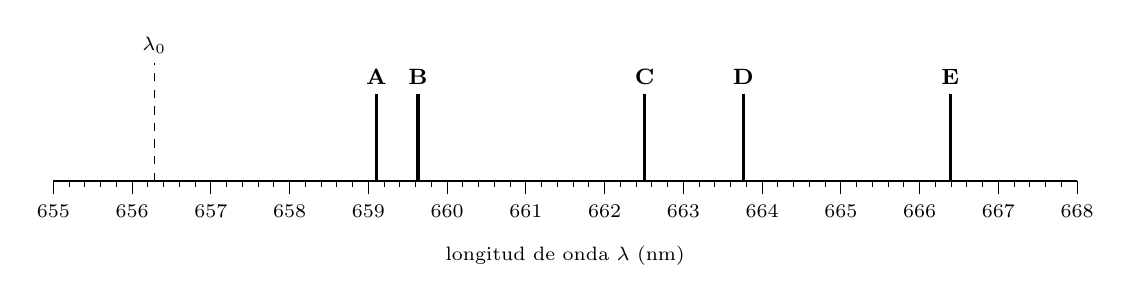
\begin{tikzpicture}[x=1cm,y=1cm]
  \draw[thick] (0,0)--(13,0);
  \foreach \m in {0,0.2,...,13}{\draw (\m,0)--(\m,-0.07);}
  \foreach \n in {655,656,...,668}{\draw ({\n-655},0)--({\n-655},-0.16); \node[below,font=\scriptsize] at ({\n-655},-0.18){\n};}
  \draw[dashed] (1.28,0)--(1.28,1.5); \node[above,font=\scriptsize] at (1.28,1.5){$\lambda_0$};
  \draw[very thick] (4.10,0)--(4.10,1.1); \node[above,font=\footnotesize\bfseries] at (4.10,1.1){A};
  \draw[very thick] (4.63,0)--(4.63,1.1); \node[above,font=\footnotesize\bfseries] at (4.63,1.1){B};
  \draw[very thick] (7.51,0)--(7.51,1.1); \node[above,font=\footnotesize\bfseries] at (7.51,1.1){C};
  \draw[very thick] (8.76,0)--(8.76,1.1); \node[above,font=\footnotesize\bfseries] at (8.76,1.1){D};
  \draw[very thick] (11.39,0)--(11.39,1.1); \node[above,font=\footnotesize\bfseries] at (11.39,1.1){E};
  \node[below,font=\scriptsize] at (6.5,-0.7){longitud de onda $\lambda$ (nm)};
\end{tikzpicture}
\end{center}

{\footnotesize Ejemplo (galaxia NGC 4639): si $\lambda_{obs}=658{,}51$ nm, entonces $\Delta\lambda=2{,}23$ nm, $z=0{,}0034$ y $v\approx1\,019$ km/s.}

\medskip
{\renewcommand{\arraystretch}{2.2}
\noindent\begin{tabular}{|l|c|c|c|c|}\hline
\textbf{Galaxia} & $\lambda_{obs}$ (nm) & $\Delta\lambda$ (nm) & $z=\Delta\lambda/\lambda_0$ & $v=c\,z$ (km/s) \\ \hline
A (NGC 3370) & & & & \\ \hline
B (NGC 3021) & & & & \\ \hline
C (NGC 5468) & & & & \\ \hline
D (IC 5179) & & & & \\ \hline
E (NGC 4679) & & & & \\ \hline
\end{tabular}}

\hojatrabajo{3 · Explore}
{\footnotesize \textbf{Construye el diagrama de Hubble.} Representa cada galaxia (distancia $d$, velocidad $v$) en la cuadrícula. Traza la recta que mejor se ajuste a las galaxias \textbf{lejanas} ($v>3\,000$ km/s; las cercanas se desvían por su movimiento propio) y estima su pendiente $H_0=v/d$.}

\medskip
{\footnotesize
\noindent\begin{tabular}{|l|r|r||l|r|r|}\hline
\textbf{Galaxia} & $d$ (Mpc) & $v$ (km/s) & \textbf{Galaxia} & $d$ (Mpc) & $v$ (km/s) \\ \hline
NGC 4536 & 14,9 & 1\,808 & NGC 4679 & 58,3 & 4\,611 \\ \hline
NGC 1316 & 17,8 & 1\,760 & UGC 00646 & 66,4 & 5\,318 \\ \hline
NGC 1380 & 18,5 & 1\,877 & Coma (4889/74) & 94,0 & 6\,895 \\ \hline
NGC 4639 & 22,1 & 1\,018 & UGC 12133 & 110,0 & 7\,423 \\ \hline
NGC 3021 & 26,8 & 1\,541 & UGC 01993 & 113,0 & 8\,019 \\ \hline
NGC 3370 & 27,4 & 1\,279 & UGC 07934 & 149,0 & 9\,624 \\ \hline
IC 5179 & 43,3 & 3\,421 & UGC 12071 & 153,0 & 10\,372 \\ \hline
NGC 5468 & 43,8 & 2\,842 & & & \\ \hline
\end{tabular}}

\medskip
\begin{center}
\begin{tikzpicture}
  \foreach \d in {0,20,...,160}{\pgfmathsetmacro\xx{\d*0.075}\draw[gray!35] (\xx,0)--(\xx,8); \node[below,font=\scriptsize] at (\xx,0){\d};}
  \foreach \v in {0,1000,...,11000}{\pgfmathsetmacro\yy{\v/1375}\draw[gray!35] (0,\yy)--(12,\yy);}
  \foreach \v in {0,2000,...,10000}{\pgfmathsetmacro\yy{\v/1375}\node[left,font=\scriptsize] at (0,\yy){\v};}
  \draw[thick,-{Stealth}] (0,0)--(12.6,0) node[right,font=\scriptsize]{$d$ (Mpc)};
  \draw[thick,-{Stealth}] (0,0)--(0,8.6) node[above,font=\scriptsize]{$v$ (km/s)};
\end{tikzpicture}
\end{center}

\noindent Pendiente estimada: $H_0 \approx$ \underline{\hspace{3cm}} km/s/Mpc.\par\medskip
\noindent Mi conjetura (¿qué patrón ves?, ¿qué crees que significa la pendiente?):\par\vspace{3mm}
\noindent\rule{\linewidth}{0.4pt}\par\vspace{5mm}\noindent\rule{\linewidth}{0.4pt}

\hojatrabajo{4 · Explain}
{\footnotesize \textbf{Calcula la edad del universo.} La edad se estima como $t\approx 1/H_0$. Para que $1/H_0$ dé un tiempo, hay que pasar los Mpc a km y los segundos a años. Sigue el \textbf{ejemplo} ($H_0=70$) y calcula \textbf{el tuyo}.}

\medskip
{\renewcommand{\arraystretch}{2.2}
\noindent\begin{tabularx}{\linewidth}{|>{\raggedright\arraybackslash}p{5.4cm}|>{\raggedright\arraybackslash}p{3.9cm}|>{\raggedright\arraybackslash}X|}\hline
\textbf{Paso} & \textbf{Ejemplo ($H_0=70$)} & \textbf{El tuyo ($H_0=$\,\rule{1.4cm}{0.4pt})} \\ \hline
$t(\text{s})=\dfrac{3{,}086\times10^{19}}{H_0}$ & $\approx 4{,}41\times10^{17}$ s & \\ \hline
$t(\text{años})=\dfrac{t(\text{s})}{3{,}156\times10^{7}}$ & $\approx 1{,}40\times10^{10}$ años & \\ \hline
En miles de millones de años & $\approx 14\,000$ & \\ \hline
\end{tabularx}}

\vspace{9mm}
\noindent\textbf{Interpreta:} ese número es una edad: ¿\textbf{la edad de qué}? ¿Y cómo lo sabes? (piensa en \emph{rebobinar} la expansión). ¿Qué \textbf{simplifica} esa fórmula sobre la expansión, que en realidad ha cambiado con el tiempo?
\par\vspace{2mm}\noindent\rule{\linewidth}{0.4pt}\par\vspace{5mm}\noindent\rule{\linewidth}{0.4pt}
\par\smallskip
{\footnotesize (En \textbf{Elaborate} verás cuánto puede cambiar esta estimación y por qué.)}

\hojatrabajo{5 · Elaborate}
\noindent\textbf{¿Hasta dónde puede llegar la luz? El ritmo de expansión \textnormal{(ampliación opcional, no evaluable)}.}
{\footnotesize En el modelo de la expansión, en cada paso la luz \textbf{avanza 1} (su velocidad; 1 unidad $\approx$ 1400 millones de años-luz, lo que recorre en un paso de $\sim$1400 millones de años) y el espacio \textbf{estira} toda distancia un ritmo $r$ (un \%, \textbf{proporcional} a la distancia). Un fotón que parte de una distancia $D$ \textbf{nos llega} solo si la expansión no supera su avance. En el caso límite la distancia no cambia: $(D-1)(1+r)=D$, de donde el \textbf{ritmo máximo} que aún deja llegar la luz es}
\[ r_{\max}=\frac{1}{D-1}. \]
\noindent Para cada objeto, calcula $r_{\max}$ y decide si su luz nos llega con el ritmo real ($\approx$10\,\%). Recuerda: $1$ unidad $\approx$ 1400 Mal, y ese 10\,\% \emph{no es arbitrario}: en un paso de $\sim$1400 M de años el universo crece de verdad $\sim$10\,\% ($1400/14\,000\approx0{,}1$, con $1/H_0\approx14\,000$ M de años).

\medskip
{\renewcommand{\arraystretch}{2.2}
\noindent\begin{tabularx}{\linewidth}{|X|c|c|>{\centering\arraybackslash}p{2.4cm}|}\hline
\textbf{Objeto (distancia hoy)} & $r_{\max}=\dfrac{1}{D-1}$ & \textbf{en \%} & \textbf{¿llega con el 10\,\%?} \\ \hline
Galaxia lejana ($D=6$, $6\times1400=8400$ Mal) & & & \\ \hline
En el horizonte ($D=11$, $11\times1400=15\,400$ Mal) & & & \\ \hline
Galaxia lejanísima ($D=21$, $21\times1400=29\,400$ Mal) & & & \\ \hline
\end{tabularx}}

\vspace{7mm}
\noindent\textbf{Interpreta:} cuanto más lejos está el objeto, ¿su ritmo máximo es \textbf{mayor} o \textbf{menor}? ¿A partir de qué distancia deja de llegarnos su luz con el 10\,\% real? Esa frontera es el \textbf{horizonte del modelo} ($15\,400$ Mal), \textbf{entre} el radio de Hubble ($\sim$14\,000) y el \textbf{horizonte de sucesos real} ($\sim$16\,000 Mal).
\par\vspace{2mm}\noindent\rule{\linewidth}{0.4pt}\par\vspace{5mm}\noindent\rule{\linewidth}{0.4pt}

\vspace{6mm}
\noindent\textbf{Debate en grupo: ¿más rápido que la luz?} Una galaxia más allá del horizonte se aleja de nosotros \textbf{más deprisa que la luz}, y por eso la luz que emite \textbf{hoy} nunca nos llegará. ¿Contradice esto la relatividad, que dice que \textbf{nada} puede ir más rápido que la luz? Discutidlo y anotad vuestra conclusión.
\par\vspace{2mm}\noindent\rule{\linewidth}{0.4pt}\par\vspace{5mm}\noindent\rule{\linewidth}{0.4pt}

\hojatrabajo{6 · Evaluate}
{\footnotesize \textbf{Verdadero o falso.} Marca V o F en cada afirmación. Entrégala y, después, compruébalas en la app (verás por qué).}

\vspace{8mm}
{\renewcommand{\arraystretch}{1.15}%
\newcommand{\vfila}[1]{\begin{minipage}[c][11mm][c]{\linewidth}\raggedright #1\end{minipage}}%
\noindent\begin{tabularx}{\linewidth}{|>{\centering\arraybackslash}m{0.8cm}|X|>{\centering\arraybackslash}m{1.5cm}|}\hline
\# & \textbf{Afirmación} & \textbf{V\quad F} \\ \hline
1 & \vfila{Que el cielo nocturno sea oscuro contradice la imagen de un universo eterno, estático y uniformemente lleno de estrellas.} & $\square$\quad$\square$ \\ \hline
2 & \vfila{El universo observable es todo el universo que existe.} & $\square$\quad$\square$ \\ \hline
3 & \vfila{Que todas las galaxias se alejen de nosotros significa que la Tierra está en el centro del universo.} & $\square$\quad$\square$ \\ \hline
4 & \vfila{El corrimiento al rojo de las galaxias lejanas se debe a que el espacio se estira mientras su luz viaja, no a un Doppler corriente.} & $\square$\quad$\square$ \\ \hline
5 & \vfila{La expansión del universo no afecta a los sistemas unidos por la gravedad, como una galaxia o el Sistema Solar.} & $\square$\quad$\square$ \\ \hline
6 & \vfila{$1/H_0$ es el tiempo que ha tardado en llegarnos la luz de una galaxia.} & $\square$\quad$\square$ \\ \hline
7 & \vfila{La materia oscura y la energía oscura son dos nombres para la misma cosa.} & $\square$\quad$\square$ \\ \hline
8 & \vfila{La ciencia ya conoce con total certeza y sin ningún debate el valor de la constante de Hubble.} & $\square$\quad$\square$ \\ \hline
9 & \vfila{Ninguna galaxia puede alejarse de nosotros más deprisa que la luz.} & $\square$\quad$\square$ \\ \hline
\end{tabularx}}

\vspace{9mm}
\noindent\textbf{En grupo: el error que enseña.} Las afirmaciones \textbf{falsas} de arriba son ideas erróneas frecuentes. Elegid una y debatid \textbf{por qué falla}: en ciencia, entender \emph{por qué} algo es falso vale tanto como saber lo correcto.

\medskip
\noindent Afirmación falsa elegida (n.\textsuperscript{o}): \underline{\hspace{1.4cm}}
\par\smallskip
\noindent ¿Por qué resulta creíble a primera vista?
\par\vspace{2mm}\noindent\rule{\linewidth}{0.4pt}\par\vspace{5mm}\noindent\rule{\linewidth}{0.4pt}
\par\smallskip
\noindent ¿Por qué es en realidad falsa? (la idea correcta y en qué os apoyáis)
\par\vspace{2mm}\noindent\rule{\linewidth}{0.4pt}\par\vspace{5mm}\noindent\rule{\linewidth}{0.4pt}
\par\medskip
\noindent\textit{Puesta en común: cada grupo defiende por qué su afirmación es errónea; el resto puede matizar o rebatir.}

\hojatrabajo{7 · Evaluate}
{\footnotesize \textbf{Producto final y autoevaluación.} \textbf{Tarea:} explica a otra persona cómo hemos medido la edad y el tamaño del universo. Elige el formato (presentación, póster o vídeo). Reconstruye la cadena $z\rightarrow v\rightarrow H_0\rightarrow$ edad $\rightarrow$ tamaño y no olvides los matices (observable $\neq$ total; $1/H_0$ es aproximado).}

\medskip
\noindent\textbf{Autoevaluación (Rúbrica B, Tabla~\ref{tab:rubricaB}).} Marca tu nivel en cada dimensión:

\medskip
{\renewcommand{\arraystretch}{1.6}
\noindent\begin{tabular}{|l|c|c|c|c|}\hline
\textbf{Dimensión} & 1 & 2 & 3 & 4 \\ \hline
Rigor conceptual & $\square$ & $\square$ & $\square$ & $\square$ \\ \hline
Explicación del proceso & $\square$ & $\square$ & $\square$ & $\square$ \\ \hline
Naturaleza de la ciencia & $\square$ & $\square$ & $\square$ & $\square$ \\ \hline
Uso de la evidencia & $\square$ & $\square$ & $\square$ & $\square$ \\ \hline
Claridad y formato & $\square$ & $\square$ & $\square$ & $\square$ \\ \hline
\end{tabular}}

\medskip
\noindent\textbf{Puntuación total} (suma de las cinco dimensiones, de 5 a 20): \underline{\hspace{3cm}}\ /\,20

\medskip
\noindent ¿Qué mejorarías si lo hicieras otra vez?\par\vspace{3mm}
\noindent\rule{\linewidth}{0.4pt}\par\vspace{5mm}\noindent\rule{\linewidth}{0.4pt}

